\documentclass[lettersize,journal]{IEEEtran}
\usepackage{booktabs} 
\usepackage{multirow}
\usepackage{subcaption}
\usepackage{stfloats}
% \usepackage{caption}
\usepackage{amsmath,amsfonts}
\usepackage{algorithmic}
\usepackage{algorithm}
\usepackage{array}
\usepackage{graphicx}
\usepackage[caption=false,font=normalsize,labelfont=sf,textfont=sf]{subfig}
\usepackage{textcomp}
\usepackage{stfloats}
\usepackage{url}
\usepackage{verbatim}
\usepackage{graphicx}
\usepackage{cite}
\hyphenation{op-tical net-works semi-conduc-tor IEEE-Xplore}
% updated with editorial comments 8/9/2021

\begin{document}

\title{Action-Dynamics Modeling and Cross-Temporal Interaction\\ for Online Action Understanding }
\author{Xinyu Yang, Zheheng Jiang, Feixiang Zhou, Yihang Zhu, Na Lv, Nan Xing and Huiyu Zhou

% \author{IEEE Publication Technology,~\IEEEmembership{Staff,~IEEE,}
        % <-this % stops a space
\thanks{X. Yang, Z. Jiang, Y. Zhu and H. Zhou are with School of Computing and Mathematical Sciences, University of Leicester, United Kingdom. H. Zhou is the corresponding author. E-mail:hz143@leicester.ac.uk.}% <-this % stops a space
\thanks{F. Zhou is with School of Eye and Vision Sciences, University of Liverpool, United Kingdom.}
\thanks{N. Lv is with School of Information Science and Engineering, University of Jinan, China.}
\thanks{N. Xing is with School of Automation and Information Engineering, Xi'an University of Technology, China.}
}


% The paper headers
\markboth{Journal of \LaTeX\ Class Files,~Vol.~14, No.~8, August~2021}%
{Shell \MakeLowercase{\textit{et al.}}: A Sample Article Using IEEEtran.cls for IEEE Journals}

% \IEEEpubid{2021}
% Remember, if you use this you must call \IEEEpubidadjcol in the second
% column for its text to clear the IEEEpubid mark.

\maketitle

\begin{abstract}
Action understanding, encompassing action detection and anticipation, plays a crucial role in numerous practical applications. However, untrimmed videos are often characterized by substantial redundant information and noise. Moreover, in modeling action understanding, the influence of the agent's intention on the action is often overlooked. Motivated by these issues, we propose a novel framework called the State-Specific Model (SSM), designed to unify and enhance both action detection and anticipation tasks. In the proposed framework, the Critical State-Based Memory Compression module compresses frame sequences into critical states, reducing information redundancy. The Action Pattern Learning module constructs a state-transition graph with multi-dimensional edges to model action dynamics in complex scenarios, on the basis of which potential future cues can be generated to represent intention. Furthermore, our Cross-Temporal Interaction module models the mutual influence between intentions and past as well as current information through cross-temporal interactions, thereby refining present and future features and ultimately realizing simultaneous action detection and anticipation. Extensive experiments on multiple benchmark datasets—including EPIC-Kitchens-100, THUMOS'14, TVSeries, and the introduced Parkinson's Disease Mouse Behaviour (PDMB) dataset—demonstrate the superior performance of our proposed framework compared to other state-of-the-art approaches. These results highlight the importance of action dynamics learning and cross-temporal interactions, laying a foundation for future action understanding research.
\end{abstract}

\begin{IEEEkeywords}
Action anticipation, Action detection, Action understanding.
\end{IEEEkeywords}

\section{Introduction} 
\IEEEPARstart{A}{ction} understanding—specifically online action detection \cite{de2016online} and action anticipation\cite{kitani2012activity}—aims to identify current or predict future actions from streaming videos. For the online task, only current and historical information can be utilized, whereas future information is inaccessible. These tasks are fundamental in action retrieval\cite{li2024adaptive}, intelligent surveillance \cite{xia2023exploring}, embodied intelligence (e.g., human–robot interaction \cite{song2018temporal}\cite{li2021restep}), and autonomous driving systems \cite{liu2023hcm}. % For example, accurately detecting human actions enables household robots to provide timely support to human users, while reliably predicting pedestrian intentions is critical for ensuring robust safety in fully automated driving \cite{rasouli2021bifold,kong2022human}. Moreover, an anomaly alert system can trigger preventative measures if anticipated actions deviate from the expected sequences.
Humans often imagine future events based on past experiences. This process can be viewed as modeling past actions to assess current or future states \cite{schacter2007remembering}. Consequently, replicating this cognitive ability is key to narrowing the performance gap between machines and humans. Current mainstream approaches predominantly center on memory mechanisms \cite{xu2021long,  chen2022gatehub, zhao2022real,  girdhar2021anticipative}. A notable example is Long Short-term TRansformer\cite{xu2021long}, which splits its memory encoder into long- and short-term stages for online action detection and anticipation, resulting in more representative memory features. Similarly, other studies have extended memory mechanism with various improvements. Temporal Smoothing Transformers \cite{chen2022gatehub} uses a streaming transformer paradigm to handle large-scale memory sequences, enabling efficient fusion of short- and long-term context to enhance memory learning and ultimately deliver strong performance in online action detection and anticipation. Gated History Unit with Background Suppression (GateHub) \cite{zhao2023learning} introduces a Gated History Unit (GHU) that applies a position-guided gated cross-attention to enhance memory segments and suppress background sequence, improving online action detection. However, during action detection or anticipation, memory-based models inevitably encounter irrelevant or distracting frames. This issue becomes more pronounced in longer videos, where redundant and noisy information accumulates over time. Consequently, critical cues may become "buried" under a flood of unrelated features, hindering the model’s ability to focus on the truly essential dependencies within the action pattern.
\begin{figure}[t]
  \centering
  % \fbox{\rule{0pt}{2in} \rule{1.8\linewidth}{0pt}}
    \includegraphics[width=1.0\linewidth]{fig/fig0.pdf}

     \caption{Comparison between Memory-Based and State-Based Methods: (a) Memory-based methods rely on learning effective representations from the entire sequence, which inevitably increases the risk of interference from redundant information and noise. (BG denotes background) (b) Our state-based method constructs ST graph to represent action dynamics. This design encourages the model to focus on the underlying dependencies between actions while suppressing the influence of redundant information and noise.}
   \label{fig2}
\end{figure}

To alleviate this issue, we propose a framework, referred to as the State-Specific Model (SSM). Compared to memory-based methods that focus on processing the entire sequence, our approach places greater emphasis on uncovering critical states embedded within the sequence. As illustrated in Fig 1, (a) Memory-based methods need to process the entire sequence to learn the potential dependencies. In contrast, (b) our state-based approach establishes critical states by using critical frames from the sequence as anchors and then models the edge between each pair of states through multi-dimensional relations, constructing a State-Transition (ST) Graph. Unlike single-valued edges that encode only one type of relation (e.g., temporal adjacency or co-occurrence patterns, etc.), our multi-dimensional edges are capable of representing multiple, distinct relationships. As suggested in \cite{gong2019exploiting}\cite{song2021learning}, this enables the modeling of richer underlying dependencies among vertices( i.e., the critical states). ST graph allows the model to focus on dynamic logic underlying action changes, without being distracted by the redundant information commonly present in long sequences. Note that the critical states we define are not tied to any critical frame; rather, they represent a collection of features that most effectively characterize the target action. 

On the other hand, when discussing action detection or anticipation, it is commonly assumed that past actions influence current or future actions; however, past actions are not the sole determining factors. In reality, actions are also typically driven by underlying intentions or goals, guiding both current and future actions. These intentions can be viewed as potential future cues. Therefore, past, present, and future actions can be viewed as mutually influential. As a result, the tasks of action detection and action anticipation are inherently complementary and interdependent. Motivated by this insight, our model leverages learned action dynamics to generate potential future cues that represent intentions. Subsequently, the model refines representations of current and future actions through interactions among past, present, and future information, thereby simultaneously enabling effective action detection and anticipation. In summary, our main contributions are as follows:
\begin{itemize}
\item We propose a novel framework called State-Specific Model (SSM), which enhances action understanding by modeling action dynamics and enabling cross-temporal interactions.
\item By introducing a temporal weighted attention mechanism, we propose the Critical State-Based Memory Compression (CSMC) module that condenses the original sequence into critical states, capturing salient information while minimizing information redundancy.
\item In the proposed Action Pattern Learning (APL) module, we model multi-dimensional transitions among these critical states to construct a ST Graph. The ST graph effectively represents action dynamics, serving as a foundation for exploring potential future cues.
\item Our Cross-Temporal Interaction (CTI) module captures the mutual influence between intentions (i.e., potential future cues) and both current and past actions through cross-temporal interactions. It updates the representations of current and future actions, thereby enabling complementary online action detection and anticipation in a unified manner.
\item Comprehensive experiments show that our SSM outperforms other state-of-the-art methods, underlining its robustness, generalizability and effectiveness  across diverse datasets.
\end{itemize}

The remainder of the paper is organized as follows. Section II reviews related work, Section III introduces the proposed method, Section IV reports the experimental results, and Section V concludes.
\section{Related Work}
\subsection{Online Action Detection}
Online Action Detection (OAD) requires identifying and classifying actions instantly, without access to future frames. Contemporary OAD methods frequently center on memory modeling to capture and leverage historical context from observed frames. Early methods primarily relied on RNN or CNN based models (e.g., \cite{deo2017learning}) to capture historical context. TRN proposed by Xu et al.\cite{xu2019temporal} explicitly modeled past frames and their temporal context, while Eun et al. \cite{eun2020learning} extended GRU \cite{cho2014learning} with a discriminative embedding model to more effectively learn representations for detecting ongoing actions. Zhao et al.\cite{zhao2022progressive} further improved learning efficiency through knowledge distillation to mitigate inconsistent visual content.

With the success of Transformers \cite{vaswani2017attention} in modeling temporal sequences, recent approaches have explored attention-based architectures. Wang et al.\cite{wang2021oadtr}, proposed an encoder-decoder framework, referred to as OadTR, to jointly encode historical information and predict future actions. LSTR proposed by Xu et al.\cite{xu2021long} expanded the memory horizon by introducing segmented memory to analyze historical context in depth. Yang et al. \cite{yang2022colar} adopted exemplary frames to guide attention scheme learning representation sothat the detection accuracy is improved. Chen et al. \cite{chen2022gatehub} introduced a gated history unit and a future-augmented background suppression strategy to better capture temporal cues. Despite these advances, OAD still faces the inherent limitation of observed information, which can reduce the effectiveness of modeling. On the other hand, current  popular methods exploit transformer's capacity for memory modeling, but the ever-growing length of the memory sequence limits the effectiveness of these methods. For the limitation of observed information, our proposed SSM employs cross-temporal interactions to facilitate richer temporal information learning. Moreover, by focusing on state-based action dynamics, our method alleviates the limitations brought by the ever-growing length of memory sequences.
\subsection{Online Action Anticipation}
Online action anticipation has received significant attention in recent years, with its primary goal being the prediction of future actions based solely on observations. Early works predominantly employed recurrent neural networks. For instance, Furnari and Farinella \cite{furnari2020rolling} utilize a Dual-LSTM structure to encode and distill input sequences, generating cyclic predictions for future frames. Their framework additionally incorporated a learnable attention module to fuse representations from RGB, optical flow, and object-centric streams, thereby capturing a wide range of visual cues. Similarly, Qi et al. \cite{qi2021self}  tackle error accumulation in recurrent models by combining a contrastive loss with an attention mechanism, iteratively refining intermediate feature embeddings. They also introduce verb and noun classification for auxiliary guidance. Subsequently, Liu and Lam \cite{liu2022hybrid} enhance the recurrent pipeline with an external memory bank and a classification loss for observed content, while employing contrastive learning to more closely align anticipated features with ground-truth sequences. 

Moving beyond recurrent networks, recent work has embraced Transformer architectures for action anticipation. Girdhar and Grauman \cite{girdhar2021anticipative} developed the Anticipative Video Transformer (AVT), combining a Transformer encoder on raw video frames with a masked decoder to jointly predict intermediate and final representations. Osman et al. \cite{osman2021slowfast} took inspiration from action recognition and devised a dual-stream approach with different frame sampling rates, aiming to capture both slow and fast dynamics in videos. Meanwhile, Roy et al. \cite{roy2024interaction} focused on human-object interactions, showing that modeling object-specific cues through attention or Transformer modules can effectively reveal which items are likely to be involved in upcoming activities. Most of the previous works have tended to focus solely on the single-task setting of action anticipation, overlooking a key aspect: The outcomes of online action detection and action anticipation mutually influence each other. Consequently, they miss the potential benefit of integrating complementary features from both tasks. Such complementarity may yield richer and more robust feature representations, which have the potential to guide the model to produce more accurate detection and anticipation results. Building on this insight, Our SSM addresses this limitation by enabling joint training or inference for both tasks simultaneously.
\vspace{-5pt}
\section{Method}
% \subsection{Architecture Overview}
\begin{figure*}[htbp]
  \centering
  % \fbox{\rule{0pt}{2in} \rule{\linewidth}{0pt}}
    \includegraphics[width=1.0\linewidth]{fig/fig_architecture.pdf}

   \caption{Overview of the proposed State-Specific Model. (a) Critical State-Based Memory Compression. Video sequence features are compressed into critical states. (b) Action Pattern Learning. A ST graph is constructed based on critical states to capture action dynamics, and subsequently, a Gated Graph Convolutional Network (Gated GCN) generates potential future cues from the ST graph. (c) Cross-Temporal Interaction. Temporal features interact across different time domains to update current and future features, supporting action detection and anticipation.}
   \label{fig}
\end{figure*}
The proposed method aims to enable the model to perform both action anticipation and detection within a video stream, as illustrated in  Fig. 2. In the following sections, we provide a detailed explanation of each module, outlining their specific contributions to the overall framework.
% \vspace{-3pt}
% The method proposed in this paper focuses on enabling the model to performs action anticipation and detection within a video stream. Our proposed SSM is illustrated in Fig 2. The proposed CSMC module compresses the input sequence into critical states, eliminating redundant information. The critical states are then utilized within the APL module, which constructs a ST graph. This graph proficiently captures underlying action dynamics by modeling relations between critical states. Leveraging learned action dynamics features, the model generates potential future cues to represent agent's intention. These cues are interacted with past and present action information through the CTI, which enriches representations. Ultimately, both action detection and anticipation are realized based on the output of the CTI module. In the following sections, we provide a detailed explanation of each module, outlining their specific contributions to the overall architecture.
% \subsection{Architecture Overview}
% Specifically, the video frame sequence $V$ with length $L$ is represented as $V=\left \{  v_t \right \} _{-(L-1)}^{0}$, where $v_t$ is the frame at relative time step $t$, with $t=0$ marking the current frame and $t=-(L-1)$ the oldest one in the video. For action anticipation, the model aims to predict the action $y_{n}$ after a time interval $\tau (\ge0)$ while for action detection, the model identifies the target's action $y_{n}$ at $t=0$. The action $y_{n}$ is chosen from the set $\left \{ 0,1,2,... N \right \}$ where $N$ represents the total number of action classes and 0 indicates the background. Importantly, none of these tasks relies on future information.
% The method proposed in this paper focuses on enabling the model to learn the target's action patterns and, further performs action anticipation and detection within a video stream. 
% Our proposed SSM is illustrated in Fig 2. Our proposed CSMC module processes the features from the input sequence, extracting critical states and eliminating information redundancy. This module employs a novel temporal weighted attention mechanism, effectively retaining essential information while suppressing irrelevant details. The identified critical states are then utilized within the APL module, which constructs a ST graph. This graph proficiently captures underlying action dynamics by modeling transitions between critical states. Leveraging these learned patterns, the model generates potential future cues. These cues are integrated with past and present action information through the CTI, which enriches feature representations via interactions across temporal domains. Ultimately, the CTI generates refined representations, thereby realizing both action detection and anticipation.
% In the following sections, we provide a detailed explanation of each module, outlining their specific contributions to the overall architecture.
\vspace{-3pt}
\subsection{Critical State-Based Memory Compression}
We use video features $F=\left \{  f_{i} \right \} _{-(L-1)}^{0}\in\mathbb{R}^{L\times D}$ as the input for our model, where $f_{i}$ denotes the single-frame feature, $F$ is video-level feature (i.e., the collection of $f$), $D$ represents the feature dimensionality and $L$ stands for the sequence length. Here, we define $F _{m}=\left \{  f \right \} _{-L_{m}}^{-1}\in \mathbb{R}^{L_{m}\times D} $ as the memory sequence, and $F _{current}=\left \{  f \right \} _{0}$ as the current frame. For the memory sequence, as it is typically a long token sequence, it may contain much redundancy. In order to allieviate this issuse, we propose the CSMC module. Firstly, we introduce a critical memory frame extraction approach based on the integration of ProPos \cite{huang2022learning} representation learning and Gaussian Mixture Models (GMM). Our approach consists of two primary stages: (1)Video Frame Clustering via ProPos-GMM;(2)Critical Memory Frame Selection. For (1), each frame feature from the memory sequence is passed through the ProPos framework to obtain discriminative and clustering-friendly feature representations. Subsequently, a GMM is applied to these learned features to cluster the video frames. Specifically, given the updated representation $f(x_{i} )$ for the $i-th$ video frame, the probability density is modeled as: 
\begin{equation}
  p(f(x_{i} ))=\sum_{k=1}^{K} \pi _{k} \mathcal{N}(f(x_{i} )\mid \mu_{k},  \Sigma_k  )
  \label{1}
\end{equation}
where $K$ is the predefined number of clusters, $\mu_{k}$ and $\Sigma_k$ denote the mean and covariance of the $k-th$ Gaussian component, respectively, and $\pi _{k}$ is the corresponding mixture coefficient automatically estimated through the Expectation-Maximization (EM) \cite{dempster1977maximum}. The posterior probability that the $i-th$ frame belongs to cluster $k$ is computed by:
\begin{equation}
    p(k\mid f(x_{i} ))=\frac{\pi _{k} \mathcal{N}(f(x_{i} )\mid \mu_{k},  \Sigma_k  )}{\sum_{j=1}^{K} \pi _{j} \mathcal{N}(f(x_{i} )\mid \mu_{j},  \Sigma_j  )}
  \label{2}
\end{equation}

After clustering, step (2) is performed. For each cluster center ($\mu_{k}$), we select the most representative frame for each cluster as the critical memory frame. Specifically, the critical memory frame $x_{k}^{c} $ for the $k-th$ cluster is selected based on the minimal Euclidean distance in the representation space to the cluster center, i.e., $x_{k}^{c} =arg\underset{x_{i} }{\min}\parallel f(x_{i} )-\mu_{k} \parallel_{2}$. Next we integrate these critical memory frames with the current frame to form the critical frames, which includes $K+1$ frames. Finally, the set of selected critical frames is obtained as: $\mathcal{C}= \left \{   x_{1}^{c},x_{2}^{c},..., x_{K}^{c},x_{K+1}^{c}\right \}$.
% \begin{equation}
%     x_{k}^{c} =arg\underset{x_{i} }{\min}\parallel f(x_{i} )-\mu_{k} \parallel_{2}  
%   \label{3}
% \end{equation}
% \begin{equation}
%     \mathcal{C}= \left \{   x_{1}^{c},x_{2}^{c},..., x_{K}^{c},x_{k+1}^{c}\right \}   
%   \label{4}
% \end{equation}

Although the extracted critical frames may capture significant moments of action occurrences within video sequences, solely relying on these frames results in sparse representations, potentially overlooking essential contextual information or potential temporal dependencies. 
% Consequently, the model fails to capture sufficient information, hindering its ability to make accurate decisions. 
To address this limitation, we propose a novel Temporal Weighted Attention (TWA) mechanism, which dynamically adjusts the attention distribution across the video sequence by incorporating temporal and relevance around critical frames. Specifically, in our TWA, the extracted critical frames serve as queries $(Q)$, while the original sequential frames act as keys $(K)$ and values $(V)$. To explicitly model temporal proximity, we introduce a temporal weighting function $g(\bigtriangleup t_{i,j} )$, where $\bigtriangleup t_{i,j} $ represents the temporal distance between the $i$-th critical frame and the $j$-th frame in the original sequence, defined as: $\bigtriangleup t_{i,j}=\left |  \right  |t_{i} -t_{j}\left |  \right |_{2}$. The temporal weighting function is formulated as a Gaussian kernel:$g(\bigtriangleup t_{i,j} )=exp(-\frac{\bigtriangleup t_{i,j}}{2\delta ^{2} } ) $, where $\delta$  is a scaling parameter controlling the sharpness of the temporal weighting distribution around the critical frames.
% \begin{equation}
%   g(\bigtriangleup t_{i,j} )=exp(-\frac{\bigtriangleup t_{i,j}}{2\delta ^{2} } ) 
%   \label{5}
% \end{equation}
 % where $\delta$  is a scaling parameter controlling the sharpness of the temporal weighting distribution around the critical frames.
The final attention weights, integrating both semantic similarity and temporal proximity, are computed as: $a_{i,j}= \sigma(\frac{Q_{i}\cdot K_{j}^{\top } }{\sqrt{d_{k}} }\cdot g(\bigtriangleup t_{i,j} )))$, where $\sigma(\cdot)$ denotes Softmax function, and $d_{k}$ is the dimensionality of the query and key vectors.
% \begin{equation}
%   a_{i,j}= \sigma(\frac{Q_{i}\cdot K_{j}^{\top } }{\sqrt{d_{k}} }\cdot g(\bigtriangleup t_{i,j} ))) 
%   \label{6}
% \end{equation}
% where $\sigma(\cdot)$ denotes Softmax function, and $d_{k}$ is the dimensionality of the query and key vectors.
The corresponding critical state representation $S_{i}$, obtained for the $i$-th critical frame, is calculated as:
% \begin{align}
% S_{i} &= \sum_{j=1}^{L} a_{ij} V_{j} \notag \\
% &= \sum_{j=1}^{L} 
% \frac{
% \exp\left(-\frac{g(\bigtriangleup t_{i,j})}{2\delta ^{2}} \right) 
% \cdot \exp\left(\frac{Q_{i} K_{j}^{\top }}{\sqrt{d_{k}}} \right)
% }{
% \sum_{j=1}^{L} 
% \exp\left(-\frac{g(\bigtriangleup t_{i,j})}{2\delta ^{2}} \right) 
% \cdot \exp\left(\frac{Q_{i} K_{j}^{\top }}{\sqrt{d_{k}}} \right)
% }
% V_{j}
% \end{align}
\begin{equation}
\scalebox{0.87}{$
S_{i} = \sum_{j=1}^{L} a_{ij} V_{j} = \sum_{j=1}^{L} 
\frac{
\exp\left(-\frac{g(\bigtriangleup t_{i,j})}{2\delta ^{2}} \right) 
\cdot \exp\left(\frac{Q_{i} K_{j}^{\top }}{\sqrt{d_{k}}} \right)
}{
\sum_{j=1}^{L} 
\exp\left(-\frac{g(\bigtriangleup t_{i,j})}{2\delta ^{2}} \right) 
\cdot \exp\left(\frac{Q_{i} K_{j}^{\top }}{\sqrt{d_{k}}} \right)
}
V_{j}
$}
\label{eq:attention}
\end{equation}

Here, the temporal weighting mechanism dynamically adjust the attention distribution based on temporal differences, enabling the model to prioritize local information around the critical frames. Simultaneously, the model retains awareness of global context, focusing on distant frames that may still provide valuable information. This dual capability allows temporal weights to effectively balance local feature extraction with broader contextual understanding. By emphasizing important details near the critical frames while not overlooking globally relevant data, the CSMC achieves a refined representation that combines precise local insights with a comprehensive view of the overall scene. Ultimately, using the TWA, we compress the input video sequence into $K+1$ critical states. Each critical state represents a contextualized action representation anchored by a critical frame. Thus, critical states not only highlight significant action-related moments but also embed rich, contextually relevant information across the entire temporal sequence. 
% This comprehensive representation serves as a robust foundation for subsequent action modeling and understanding tasks.
% \vspace{-3pt}
% \subsection{Action Pattern Learning}
% \begin{figure}[htbp]
%   \centering
%   % \fbox{\rule{0pt}{2in} \rule{0.9\linewidth}{0pt}}
%     \includegraphics[width=1.0\linewidth]{fig/fig_graph.pdf}
%    \caption{Illustration of State-Transition Graph construction in the APL module. }
%    \label{fig3}
% \end{figure}
% \begin{figure}[t]
%   \centering
%   % \fbox{\rule{0pt}{2in} \rule{0.9\linewidth}{0pt}}
%     \includegraphics[width=1.0\linewidth]{fig/fig_states.pdf}

%    \caption{Illustration of the rationale for fully connected edges between critical states when constructing the state-transition graph. Circles of different colors represent critical states constructed using the critical frames above them as anchors. (Top) A video sequence contains multiple temporally related actions. (a) Simply connecting critical states according to the temporal order of their critical frames may overlook significant semantic dependencies (e.g. second \textit{open cupboard}). (b) Employing edges encoded by a single scalar value restricts the model to capturing only simple temporal relationships (e.g., adjacency), ignoring logical but temporally distant relationships, such as the fact that \textit{close cupboard} logically follows \textit{open cupboard}, despite temporal separation. Thus, the potential dependency between closing a cupboard and opening a cupboard may be overlooked.(c) Our proposed approach utilizes fully connected multi-dimensional edge encoding, enabling the model to capture more diverse action dynamics, thus revealing intricate dependencies beyond mere temporal adjacency.}
%    \label{fig2}
% \end{figure}
% \begin{figure}[htbp]
%   \centering
%   % \fbox{\rule{0pt}{2in} \rule{0.9\linewidth}{0pt}}
%     \includegraphics[width=1.0\linewidth]{fig/fig_graph.pdf}
%    \caption{Illustration of State-Transition Graph construction in the APL module. }
%    \label{fig3}
% \end{figure}
\vspace{-3pt}
\subsection{Action Pattern Learning}
\begin{figure}[htbp]
  \centering
  % \fbox{\rule{0pt}{2in} \rule{0.9\linewidth}{0pt}}
    \includegraphics[width=1.0\linewidth]{fig/fig_graph.pdf}
   \caption{Illustration of State-Transition Graph construction in the APL module. }
   \label{fig3}
\end{figure}
Each critical state is anchored by a critical frame and encapsulates critical contextual information. Therefore, comprehensively modeling the relationships among critical states is crucial for accurately constructing action dynamics. We provide analyses for various scenarios, with details available in the supplementary material. Ultimately, we introduce the APL module, which captures multidimensional relationships between critical state pairs based on intrinsic logic correlations rather than solely relying on temporal proximity. Specifically, APL employs a Cross-Attention (CA) mechanism to quantify pairwise dependencies between critical states, as illustrated in Fig. 3. Mathematically, given two critical states $S_{i}$ and $S_{j}$, their mutual dependency relationships can be formulated as: $E_{i,j}, E_{j,i}=CA((S_{i}, S_{j}),(S_{j},S_{i}))$. Here, $ E_{i,j}$ and $E_{j,i}$ represent multi-dimensional transition edges between critical states $S_{i}$ and $S_{j}$. By modeling these pairwise transition relationships, we construct the State-Transition Graph, where critical states serve as nodes and the modeled multi-dimensional relations form the graph edges. Unlike conventional approaches that typically encode a single type of relationship in graph edges—such as temporal adjacency or simple co-occurrence patterns—our method employs multidimensional edges to capture diverse and rich dependencies between pairs of critical states. This design allows the graph to more comprehensively represent complex action dynamics, uncovering both explicit and implicit dependencies within the action pattern.
% \begin{equation}
%   E_{i,j}, E_{j,i}=CA((S_{i}, S_{j}),(S_{j},S_{i}))
%   \label{8}
% \end{equation}

Once the State-Transition Graph is constructed, it is processed by a Gated Graph Convolutional Network (Gated GCN) \cite{bresson2017residual}, which aggregates and propagates information across graph nodes. The Gated GCN dynamically learns the underlying action dynamics and produces a latent representation, termed the potential future cue, to represent intention. This representation offers essential anticipatory context for downstream tasks such as action detection and anticipation. Overall, the proposed APL mechanism captures complex action patterns and their temporal dynamics by leveraging the rich relational representation of critical states.
\subsection{Cross-Temporal Interaction}
   \label{fig2}
\begin{figure}[htbp]
  \centering
  % \fbox{\rule{0pt}{2in} \rule{0.9\linewidth}{0pt}}
    \includegraphics[width=0.7\linewidth]{fig/figure_cti.pdf}

   \caption{CTI simulates the interaction between the intention (potential future cue) and both present and past action information through cross-temporal interaction. This process further refines the present cue and future cue, thereby enhancing support for action detection and anticipation.}
   \label{fig3}
\end{figure}
The potential future cue derived from the ST Graph effectively captures generalized action patterns and inherently represents broad and abstract behavioral trends, making it a suitable proxy for modeling intention. However, to achieve more accurate action detection and anticipation, it is essential to refine and update these representations by simulating  mutual influence between the intention and both past and present action information. To this end, we introduce the CTI module, designed to facilitate interactions among past, present, and potential future contexts. By integrating historical action cues, current action dynamics, and anticipated future trends, CTI reconstructs the contextual relationships across different temporal features, enabling more precise and context-aware action detection and anticipation. Specifically, as shown in Fig. 4, the CTI mechanism operates on three distinct temporal feature sets: (1) Past features $F_{p} $: Historical critical states, aligned with the temporal order of critical frames, are employed to characterize the observed historical action cues; (2) Present features $F_{c} $: Immediate action dynamics aligned with current critical states, capturing ongoing actions;(3)Potential future features $F_{a} $: Action trends inferred from the State-Transition Graph, representing the agent's intention. These three temporal contexts are initially concatenated into a unified temporal representation: $F_{t}=[F_{p},F_{c},F_{a}]$, which serves as the basis for subsequent interactions. We employ cross-attention (CA) to model interactions and update the temporal representations. First, the present features $F_{c} $ are dynamically refined by attending to the combined past and future contexts: $F_{c}^{'} =CA(F_{c},F_{t},F_{t})$, yielding a refined current representation $F_{c}^{'}$ that is complemented by semantic information from both historical and anticipated temporal contexts. Subsequently, the future features are refined through a cross-attention mechanism by attending to the newly updated present features and the historical dynamics. To this end, we first concatenate the past features ($F_p$), the refined current features ($F_c^{'}$), and the potential future cue ($F_a$) to form the context set $F_{t}^{'} = [F_p, F_c^{'}, F_a]$.  The future representation is then updated via cross-attention as: $F_{a}^{'} =CA(F_{a},F_{t}^{'},F_{t})^{'}$. Finally, the updated representations, $F_{c}^{'}$ and $F_{a}^{'}$, obtained from the CTI, are fed into the classifier to generate the final predictions. This strategy ensures that both detection and anticipation outcomes benefit from enriched cross-temporal contextualization, resulting in predictions that are simultaneously precise, and contextually coherent.
% This two-stage attention process allows the CTI to leverage a bidirectional flow of temporal information. On the one hand side, the current action representation becomes more precise and contextually informed by incorporating insights from historical patterns and potential future actions. On the other hand, future anticipation cues are simultaneously guided and refined by actual observed dynamics, resulting in realistic predictions aligned closely with genuine temporal behaviors. 
% Overall, the proposed CTI mechanism achieves dual advantages: (1) enhancing the accuracy and contextual awareness of action detection by grounding present representations in both past observations and future anticipations, and (2) refining action anticipation to ensure realistic alignment with the observed temporal patterns. Consequently, the CTI provides a comprehensive cross-temporal modeling approach, effectively capturing complex and realistic temporal interactions in sequences.
\subsection{Loss Function}
To improve the accuracy of online action detection and anticipation, while enforcing logical consistency between anticipated future actions and their actual occurrences, we propose a multi-component loss function:

\textbf{Action Detection Loss $L_{d}$}: To accurately identify ongoing actions within the current frame, we employ a supervised cross-entropy (CE) loss defined as:$L_{d} =CE(y_{d},p_{d})$,where $y_{d} $ denotes the labels for current action detection, and $p_{d}$ represents the model’s predicted probability distribution for current actions.
% \begin{equation}
%   L_{d} =CE(y_{d},p_{d})
%   \label{9}
% \end{equation}

\textbf{Action Anticipation Loss $L_{a}$}:To facilitate precise anticipation of future actions, we define an anticipation loss, also employing cross-entropy, formulated as:$L_{a} =CE(y_{a},p_{a})$,where $y_{a}$ represents the future action labels, and $p_{a}$ denotes the predicted distribution of future actions. 
% \begin{equation}
%    L_{a} =CE(y_{a},p_{a})
%   \label{10}
% \end{equation}

\textbf{Logical Consistency Loss via ST Graph $L_{st}$}: To ensure logical coherence between the anticipated action distribution and the lpotential future cue, we introduce a Logical Consistency Loss based on Kullback–Leibler (KL) divergence. Specifically, we constrain the model's predicted future distribution $p(a_{a})$ to align with the distribution $p_{st}(a_{a})$ which represents the potential future cues inferred from the ST Graph. Accordingly, minimizing the loss $L_{st} =D_{KL} (p_{st}(a_{a})\parallel p(a_{a}) )$ encourages the model to produce potential future cues that are logically consistent with the actual future dynamics, thereby maintaining alignment between logical priors and predictions throughout training.
% \begin{equation}
%   L_{st} =D_{KL} (p_{st}(a_{a})\parallel p(a_{a}) )
%   \label{11}
% \end{equation}

Consequently, our complete optimization objective is a weighted combination of these three terms:$L =L_{d} +\lambda_{a}  L_{a} +\lambda_{st}L_{st} $, where $\lambda_{a}$ and $ \lambda_{st}$ are hyperparameters controlling the balance among immediate detection accuracy, future action anticipation, and logical consistency between prediction and logic priors. By jointly optimizing these terms, our method ensures that the final representations integrate accurate action detection and anticipation capabilities.
% \begin{equation}
%   L =L_{d} +\lambda_{a}  L_{a} +\lambda_{st}L_{st} 
%   \label{12}
% \end{equation}

\section{Experiments}
\subsection{Datasets and Metrics}
\textbf{Datasets.} We evaluate our proposed method on four benchmark datasets: EPIC-Kitchens-100 \cite{damen2022rescaling}, THUMOS'14 \cite{jiang2014thumos}, TVSeries \cite{de2016online}, and the Parkinson’s Disease Mouse Behaviour (PDMB) dataset \cite{zhou2024smc}, covering diverse domains and challenging scenarios. Notably, the PDMB dataset provides a valuable resource for studying behavioral patterns in mice. 

\textbf{Metrics.} For THUMOS'14, we evaluate performance using mean Average Precision (mAP). For the TVSeries dataset, we adopt the mean calibrated Average Precision (mcAP) metric \cite{de2016online}. For EPIC-Kitchens-100, we follow the evaluation protocol established in \cite{damen2022rescaling}, and report the class-mean top-5 Recall separately for verbs, nouns, and actions. For the PDMB dataset, we use both mAP and mcAP as evaluation metrics. Regarding the action anticipation task, we follow prior works\cite{damen2022rescaling} \cite{guo2024uncertainty}\cite{wang2023memory}and primarily assess model performance under an anticipation time gap of $t=1s$.Due to length limitations, details regarding the datasets, evaluation metrics, and implementation can be found in the supplementary material.
% \begin{itemize}
%     \item EPIC-Kitchens-100 \cite{damen2022rescaling}: A comprehensive first-person video dataset documenting daily kitchen activities. It comprises approximately 100 hours of video footage, featuring over 90,000 annotated action segments categorized into 97 verb classes and 300 noun classes, making it particularly suitable for evaluating both action detection and anticipation. Following previous works\cite{damen2022rescaling}\cite{wang2023memory}, our model is trained on the training set and the validation set.
%   \item THUMOS'14 \cite{jiang2014thumos}: A challenging benchmark for action detection, containing over 20 hours of sports video footage annotated with 20 distinct action categories. Our model is trained on the validation set and evaluated on the test set.
%   \item TVSeries \cite{de2016online}: This dataset includes 27 untrimmed videos on six popular TV series, divided into 13, 7, and 7 videos for training, validation, and test, respectively. The dataset is temporally annotated with 30 realistic actions (e.g., open door, read, eat, etc). 
  
% \end{itemize}

% To further validate the generalization capability and applicability of our approach in specialized contexts, we introduce the Parkinson’s Disease Mouse Behaviour (PDMB) dataset. This dataset was collaboratively collected with biologists at Queen’s University Belfast, aiming to analyze behavioral patterns of mice with Parkinson’s disease (PD). Previous studies \cite{jiang2021multi, jiang2018context, jiang2022detecting, zhou2025cross, zhou2021structured, yang2024online, zhou2024smc} have confirmed its reliability for investigating behavioral correlations associated with PD. The PDMB dataset consists of videos approximately 9-14 minutes in length, each annotated at the frame level across eight distinct action categories. In our experiments, we utilize eight videos for training and two videos for testing, enabling rigorous evaluation of our method's effectiveness within a medical-relevant, behavior-analysis scenario.

% For online action detection, we adopt standard evaluation protocols consistent with previous works such as \cite{de2016online, wang2021oadtr, xu2021long, yang2022colar}. Specifically, for the THUMOS'14, performance is assessed using mean Average Precision (mAP), a widely-used metric that effectively measures the average precision across all action classes at a specified IoU threshold. For the TVSeries dataset, due to its inherent class imbalance, we employ the mean calibrated Average Precision (mcAP) \cite{de2016online}, which adjusts performance evaluation to accurately reflect imbalanced action distributions. Additionally, on our proposed PDMB dataset, we utilize both mAP and mcAP metrics to comprehensively evaluate online action detection performance.

% For action anticipation tasks, we follow the evaluation protocol established in \cite{damen2022rescaling}. Specifically, we report the class-mean top-5 Recall scores separately for verb, noun, and action predictions at an anticipation time gap $t=1s$. This provides a robust measure of the model's capability to anticipate future actions effectively. Regarding the PDMB dataset, we similarly apply the mAP and mcAP metrics at a 1-second anticipation interval, ensuring a consistent and detailed evaluation of action anticipation performance across diverse scenarios.
% \subsection{Implementation Details.}
% For experiments conducted on the EPIC-Kitchens-100 dataset, we utilize RGB, optical flow, and object features. In contrast, for experiments on the TVSeries, THUMOS'14, and PDMB datasets, only RGB and optical flow features are employed.

% In terms of model training, we adopt the Adam optimizer with an initial learning rate of $3\times 10^{-4} $ and a weight decay of $1\times 10^{-4} $. For the temporal weighting function described in Equation (5),  we set the scaling parameter $\delta=1$. Additionally, the loss-function balancing hyperparameters $\lambda_{1}$ and $\lambda_{2}$ are empirically set to 1.1 and 0.7, respectively, effectively controlling the contributions of detection, anticipation, and logical consistency components. Experiments were conducted on the
% Sulis High-Performance Computing (HPC) platform, enabling efficient training processes and optimal computational performance.



\subsection{Ablation Study}
\begin{figure}[htbp]
  \centering
  % \fbox{\rule{0pt}{2in} \rule{2\linewidth}{0pt}}
    \includegraphics[width=1.0\linewidth]{fig/ablation.pdf}

   \caption{Ablation Experiments. We conduct detailed ablation on (a): Memory Sequence Length, (b): Cluster Number and (c): Shared Classifier, FS and US denote fully shared classifier and unshared classifier, separately.}
   \label{fig5}
\end{figure}

\begin{table}
\caption{Ablation study on the temporal information interaction in CTI. }
  \centering
  \begin{tabular}{@{}lccccc@{}}
    \toprule
    No.&Past ($F_{p}$)& Present ($F_{c}$)&Future ($F_{a}$)&Detection&Anticipation \\
    \midrule
    
    (1)&&  &  & 46.1& 43.9 \\
    (2)&\checkmark &\checkmark & &51.1 & 43.9 \\   
   (3) &\checkmark & & \checkmark&46.1 & 54.9 \\
    (4)& & \checkmark& \checkmark& 46.1&  55.8\\
   (5) &\checkmark & \checkmark&\checkmark &71.8 & 58.1 \\
    
    \bottomrule
  \end{tabular}
  
  \label{tab:example}
  
\end{table}
To thoroughly examine the effectiveness of the proposed SSM, we conduct detailed ablation experiments on the THUMOS'14 test set, analyzing critical factors including memory sequence length, number of clusters, classifier design, and temporal interactions. Following prior works \cite{xu2021long} \cite{wang2023memory}, we adopt mAP as the evaluation metric in this section.


\textbf{Memory Sequence Length.} Fig. 5 (a) investigates the effect of the memory sequence length $L_{m}$ in Critical State-based Memory Compression. Results indicate that increasing the memory sequence length initially enhances performance by providing richer temporal context and more comprehensive action cues. However, beyond an optimal threshold ($L_{m}=511$), performance begins to decline. This degradation occurs due to the inclusion of frames less relevant to the current action, introducing noise and diluting the significance of critical states. Longer sequences also increase computational complexity and hinder effective modeling of critical state relations. To balance sufficient context with computational efficiency, we set the memory sequence length to $L_{m}=511$.

\textbf{Number of Clusters.} As shown in Fig. 5 (b), model performance initially improves with an increasing number of clusters ($K$), but declines beyond an optimal value ($K=4$). Initially, additional clusters enrich the ST graph structure, allowing the model to capture meaningful action patterns. However, further increasing clusters introduces complexity, presenting several challenges: (1) The computational burden grows significantly due to processing larger graphs with numerous irrelevant or redundant connections; (2) Essential state-transition dependencies become obscured or diluted amid overly complex connections, diminishing the model's ability to identify crucial action transitions clearly; (3) With too many clusters, individual nodes contribute less significantly, leading to ambiguity and reduced predictive accuracy. To achieve optimal balance, we set cluster number $k=4$, effectively balancing representational capacity and computational efficiency.

\textbf{Shared Classifier.} Fig. 5 (c) evaluates classifier-sharing strategies between action detection and action anticipation tasks. Our results reveal that employing a fully shared classifier yields the best overall performance. The shared classifier effectively integrates diverse temporal information, benefiting from cross-temporal data augmentation and promoting richer, more robust feature representations. The unified classifier structure ensures consistency across tasks, capturing common action characteristics while preserving task-specific nuances. This cross-temporal integration significantly enhances action detection and anticipation, highlighting the importance of leveraging shared representations.


\textbf{Cross Temporal Interaction.} Table 1 analyzes the impact of interactions among the past ($F_{p}$), present ($F_{c}$), and intention (potential future, $F_{a}$) on model performance. In Case (1), without performing cross-temporal interaction, the model relies solely on the current critical state and potential future cues, yielding limited performance in both action detection ($46.1\%$) and action anticipation ($43.9\%$). In Case (2), interaction between past and present features is implemented, leading to improved action detection performance ($51.1\%$). This highlights the importance of historical context in supporting action detection. Cases (3) and (4) demonstrate that interacting future cues with either past or present features significantly enhances action anticipation performance. This underscores the value of cross-temporal interaction for effective anticipation. Notably, Case (4) outperforms Case (3), indicating that present-state features exert a stronger influence than historical ones in optimizing action anticipation. Finally, Case (5) achieves the best overall performance by interacting past, present, and future information—reaching $71.8\%$ in action detection and $58.1\%$ in action anticipation. This comprehensive design effectively captures cross-temporal dependencies, enabling dynamic and context-aware prediction refinement. These results validate the critical role of the proposed CTI module in bridging observed context and future cue. By dynamically interacting information across the temporal spectrum, the model achieves accurate and coherent action detection and anticipation.
% \begin{itemize}
%   \item Case (1), relying solely on potential future cues without observed action grounding, achieves limited anticipation performance ($43.9\%$).Similarly, Case (2), using only present features, achieves action detection performance of $46.1\%$.
%   \item In Case (3), integrating past and present features yields improved action detection performance $51.1\%$, highlighting the value of historical context in supporting accurate predictions.
%   \item Cases (4) and (5) demonstrate that incorporating future cues with either past or present features significantly enhances both detection and anticipation, indicating the complementary nature of potential future information. Moreover, Case (5) surpasses Case (4), emphasizing the stronger influence of present-state information compared to historical cues in improving predictions.
%   \item Finally, Case (6), which jointly integrates past, present, and future information, achieves the best overall performance ($71.8\%$ detection and $58.1\%$ anticipation). This holistic design effectively captures dependencies across all temporal contexts, enabling dynamic refinement of predictions.
% \end{itemize}
\subsection{Comparison with State-of-the-Art Methods}
\begin{table}
\caption{Comparison to prior work on EPIC-Kitchens-100 in terms of Action Anticipation. }
  \centering
  \begin{tabular}{@{}ccccc@{}}
    \toprule
    Method & Modality&Verb&Noun&Action \\
    \midrule
    RULSTM\cite{furnari2019would}&RGB&27.5& 29.0& 13.3\\
    AVT\cite{girdhar2021anticipative} &RGB&30.2& 31.7& 14.9\\
    TeSTra\cite{zhao2022real}& RGB&26.8& 36.2& 17.0 \\
     MeMViT\cite{wu2022memvit}& RGB&32.8&33.2&15.1\\
    MAT\cite{wang2023memory}&RGB& \underline{32.7} & \textbf{39.7}& 18.8 \\
    S-GEAR$-$2B\cite{diko2024semantically} & RGB&\underline{32.7}  &37.9 & \underline{19.6}\\
    CPM\cite{xie2024towards}& RGB& -&-& 17.2\\
    Ours& RGB& \textbf{36.8}& \underline{39.2}&\textbf{19.9}\\
    \midrule
    TeSTra\cite{zhao2022real}& RGB+OF&30.8& 35.8& 17.6 \\
    MAT\cite{wang2023memory}& RGB+OF& \underline{35.0}& \underline{38.8}& 19.5 \\
    S-GEAR$-$2B\cite{diko2024semantically}& RGB+Obj &30.5 &38.4&19.6\\
    S-GEAR$-$4B\cite{diko2024semantically} & RGB+Obj  &30.2  &37.0 & \underline{19.9}\\
    Ours& RGB+OF& \textbf{38.8}&\textbf{42.1} & \textbf{21.4}\\
    \midrule
    RULSTM\cite{furnari2019would}&RGB+OF+Obj&27.8& 30.8& 14.0\\
   AVT+\cite{girdhar2021anticipative}&RGB+OF+Obj&28.2& 32.0& 15.9\\
    CPM\cite{xie2024towards}& RGB+OF+Obj& -&-& 19.4\\
    
    UADT \cite{guo2024uncertainty}& RGB+OF+Obj &\underline{43.5}& \underline{46.6}& \underline{23.0}\\
    
    Ours& RGB+OF+Obj& \textbf{44.9}&\textbf{48.3} & \textbf{24.9}\\
    
   
    
    \bottomrule
  \end{tabular}
  
  \label{tab:example}
\end{table}

\begin{table}[ht]
\caption{Action anticipation result on THUMOS’14 and TVSeries, mAP is reported for THUMOS’14 and mcAP for TVSeries.}
\centering
\begin{tabular}{@{}lcccccc@{}}
  \toprule
  % 第一列合并2行(可选,如果需要的话)
  \multirow{2}{*}{\textbf{Method}} 
    & \multicolumn{2}{c}{\textbf{THUMOS’14}} 
    & \multicolumn{2}{c}{\textbf{TVSeries}} 
    \\
  % ---- 在这里用 \cmidrule 分别给 THUMOS’14、TVSeries、HDD 画局部横线 ----
  \cmidrule(lr){2-3}
  \cmidrule(lr){4-5}
    % 第6列到第6列,只在“HDD”下方画线

  & \textbf{Kinetics} & \textbf{ANet} 
  & \textbf{Kinetics} & \textbf{ANet} 
  &\\
  \midrule
  RED\cite{gao2017red }&-& 37.5& 75.1&- \\
    TRN \cite{xu2019temporal}&- & 38.9& 75.7&- \\
    OadTR\cite{wang2021long} &53.5 & 45.9& 77.8&79.1 \\
    Lstr   \cite{xu2021long} & 52.6&50.1 &80.8 &-  \\
    GateHUB \cite{chen2022gatehub}&- & 54.2&82.0 & -\\
    TeSTra\cite{zhao2022real}& 56.8&55.3& -& - \\
     MAT\cite{wang2023memory}& \underline{58.2}& \underline{57.3}& \underline{82.6}& \underline{81.5} \\
     HCM\cite{liu2023hcm}     &54.6 & 53.3 & 80.9 & -  \\
    Ours & \textbf{61.9}& \textbf{58.9}&\textbf{85.1}& \textbf{83.7}\\
   
  \bottomrule
\end{tabular}

\label{tab:example}
\end{table}

% \begin{table}[!htb]
% 	\caption{ Action anticipation results on the PDMB dataset.}
% 	\begin{center}		
% 		\begin{tabular}{lcc} 
% 			\toprule 
% 			Methods&mAP(\%)&mcAP(\%) \\ 
% 			\midrule 
			
% 			{LSTR\cite{xu2021long}}
% 			&\underline{49.6}&\underline{72.0}\\
% 			{OadTR\cite{wang2021oadtr}}
% 			&36.2&49.9\\
% 			{Colar\cite{yang2022colar}}
% 			&42.8&65.5\\
% 			{TeSTra\cite{zhao2022real}}
% 			&40.4&55.7\\
%             {MAT\cite{wang2023memory}}
% 			&47.3&70.9\\
            
% 			$\mathbf{Ours}$
% 			&$\mathbf{52.9}$&$\mathbf{78.7}$\\
% 			\bottomrule 			
% 		\end{tabular}
% 	\end{center} 
% \end{table}



\subsubsection{Action Anticipation}
We comprehensively compare the proposed method against recent state-of-the-art (SOTA) approaches across multiple widely recognized datasets, including the EPIC-Kitchens-100 dataset, THUMOS'14 dataset, TVSeries dataset, and our  introduced PDMB dataset.

Table II presents a detailed quantitative evaluation of our approach against several representative state-of-the-art methods on the EPIC-Kitchens-100 dataset. The class-mean Top-5 recall metrics for Verb, Noun, and Action class are reported under different modality configurations. The table is structured into three distinct modality groups: RGB-only (rows 1–8), Two-Modality features (rows 9–13), and the fully multi-modal configuration (RGB+Optical Flow+Object, rows 14–18).

\textbf{Single-Modality:} When using only RGB inputs, our method achieves a verb accuracy of 36.8\%, surpassing all previous methods, including MAT (32.7\%) and S-GEAR (32.7\%). In noun anticipation, our method obtains 39.2\%, closely approaching the state-of-the-art MAT (39.7\%) with only a marginal difference (-0.5\%). We think that this result stems from our method’s emphasis on modelling action dynamics, while its capability for fine-grained semantic understanding remains limited. Consequently, when only RGB features are supplied, SSM achieves strong verb-classification performance but lags behind on noun classification. Crucially, in overall action anticipation, our method sets a new benchmark with a performance of 19.9\%, exceeding all prior approaches such as MAT (18.8\%) and S-GEAR (19.6\%). These results clearly demonstrate our method's superior capability in modeling and leveraging RGB-only features for action anticipation.

\textbf{Two-Modality:} When introducing additional modalities to the RGB input, significant improvements in performance are observed, as shown in the middle block of Table II. Our proposed model demonstrates outstanding results by combining RGB and optical flow features, attaining verb, noun, and action anticipation performances of 38.8\%, 42.1\%, and 21.4\%, respectively. These results represent clear advancements over the strongest multi-modal methods, such as MAT (RGB+OF: verb 35.0\%, noun 38.8\%, action 19.5\%) and S-GEAR-4B (RGB+Obj: action 19.9\%), underscoring our approach's effectiveness in capturing and fusing complementary multi-modal information.

\textbf{Full Multi-Modality:} To further assess the upper-bound capability of our method, we combine all three modalities: RGB, Optical Flow, and Object features. As shown in the lower section of Table II, our approach achieves substantial gains, reaching 44.9\% in verb anticipation, 48.3\% in noun anticipation, and 24.9\% in overall action anticipation. This represents a notable performance improvement compared to the previous state-of-the-art UADT method (verb: 43.5\%, noun: 46.6\%, action: 23.0\%) under identical modality settings, further confirming our framework’s ability to capture and fuse comprehensive spatio-temporal cues effectively.

We further evaluated the proposed method against state-of-the-art approaches in terms of action anticipation task on the THUMOS’14 and TVSeries datasets. As shown in Table III, our method demonstrates improvements across all metrics. Specifically, using Kinetics-pretrained features, our approach outperforms the previous best-performing method, MAT, achieving a 3.7$\%$ improvement on THUMOS’14 (61.9$\%$ vs. 58.2$\%$) and a 2.5$\%$ improvement on TVSeries (85.1$\%$ vs. 82.6$\%$). Similarly, with ActivityNet-pretrained features, our method achieves consistent gains, surpassing MAT by 1.6$\%$ on THUMOS’14 (58.9$\%$ vs. 57.3$\%$) and by 2.2$\%$ on TVSeries (83.7$\%$ vs. 81.5$\%$).These consistent improvements underline the robustness of our framework across various contexts. To evaluate the generalization capability of the proposed method, we also assess its action anticipation performance on the PDMB dataset. The results demonstrate the generalization ability of the proposed method for action anticipation. Due to space limitations, details are provided in the supplementary material.

% In order to test the generalization ability of the proposed method, we evaluate the proposed method on the PDMB dataset. The results of the action anticipation task on the PDMB dataset, presented in Table IV, highlight the superiority of our proposed method. Our approach achieves a mAP of 52.9\% and an mcAP of 78.7\%, surpassing previous methods such as MAT and LSTR, respectively. Compared to these previous methods, which also struggle with memory sequence where the action is subtle, our action-pattern-based approach demonstrates significant improvements. The ability of our method to reduce redundancy while focusing on representative moments makes it particularly suitable for scenarios requiring fine-grained action recognition, such as Parkinson’s disease mouse behavior analysis. These results reinforce the effectiveness of our framework in capturing subtle details, demonstrating the generalization ability of the proposed method in terms action anticipation. These results highlight the effectiveness of our proposed framework in terms of anticipation performance. Also, the results further demonstrate the model’s capability to generalize across diverse datasets for precise anticipation.
\begin{table}[ht]
\caption{Online action detection performances on THUMOS’14 and TVSeries.}
\centering
\begin{tabular}{@{}lccccccc@{}}
  \toprule
  % 第一列合并2行(可选,如果需要的话)
  \multirow{2}{*}{\textbf{Method}} 
    & \multicolumn{2}{c}{\textbf{THUMOS’14}} 
    & \multicolumn{2}{c}{\textbf{TVSeries}} 
    \\
  % ---- 在这里用 \cmidrule 分别给 THUMOS’14、TVSeries、HDD 画局部横线 ----
  \cmidrule(lr){2-3}
  \cmidrule(lr){4-5}
    % 第6列到第6列,只在“HDD”下方画线

  & \textbf{Kinetics} & \textbf{ANet} 
  & \textbf{Kinetics} & \textbf{ANet} 
  &\\
  \midrule
  TRN\cite{xu2019temporal}&62.1&47.2&86.2&83.7\\
  OadTR\cite{wang2021long}&65.2&58.3&87.2&85.41 \\
  Colar  \cite{yang2022colar} & 66.9 & 59.4 & 88.1 & 86.0  \\
  Lstr   \cite{xu2021long} & 69.5 & 65.3 & 89.1 & 88.1 \\
  GateHUB \cite{chen2022gatehub}& 70.7 & 69.1 & 89.6 & 88.4  \\
  TeSTra\cite{zhao2022real}  & \underline{71.2} & 68.2 &   -   &    -  \\
   MAT\cite{wang2023memory}     & 71.6 & \underline{70.4} & \underline{89.7} & \underline{88.6}  \\
   HCM\cite{liu2023hcm}     & 68.7 & 66.2 & 88.2 & -  \\
  ADI-Diff\cite{foo2024action}& 70.8  &  - & -  & -  &  \\
  ContextDet\cite{wang2024contextdet}&69.5&  -    &  - &  - &  \\  
  Ours    & \textbf{72.1} & \textbf{71.8} 
          & \textbf{90.4} & \textbf{89.8} 
          \\
  \bottomrule
\end{tabular}

\label{tab:example}
\end{table}
\begin{table}
\caption{Online action detection result on EPIC-Kitchens-100. Accuracy is measured by class-mean top 5 recall}
  \centering
  \begin{tabular}{@{}llccc@{}}
    \toprule
    Method &Verb&Noun&Action \\
    \midrule
    Lstr   \cite{xu2021long}&39.6& 44.1& 22.6 \\
    TeSTra\cite{zhao2022real}&40.0& 44.8& 23.2 \\
    MAT\cite{wang2023memory}& 41.8& 46.1& 24.9 \\
    MAT-MC\cite{wang2023memory}& \underline{44.5}& \underline{48.3}& \underline{26.3} \\
    
    
    Ours & \textbf{49.4}& \textbf{51.9}&\textbf{30.6}\\
    
   
    
    \bottomrule
  \end{tabular}
  
  \label{tab:example}
\end{table}
% \begin{table}[!htb]
% 	\caption{ Action detection results on the PDMB dataset.}
% 	\begin{center}		
% 		\begin{tabular}{lcc} 
% 			\toprule 
% 			Methods&mAP(\%)&mcAP(\%) \\ 
% 			\midrule 
			
% 			{LSTR\cite{xu2021long}}
% 			&57.4&86.9\\
% 			{OadTR\cite{wang2021oadtr}}
% 			&58.9&87.4\\
% 			{Colar\cite{yang2022colar}}
% 			&\underline{59.8}&\underline{88.6}\\
% 			{TeSTra\cite{zhao2022real}}
% 			&45.1&76.3\\
%             {MAT\cite{wang2023memory}}
% 			&58.8&87.2\\
            
% 			$\mathbf{Ours}$
% 			&$\mathbf{65.2}$&$\mathbf{94.9}$\\
% 			\bottomrule 			
% 		\end{tabular}
% 	\end{center} 
% \end{table}
\subsubsection{Action Detection}.
We validate our proposed method on the online action detection task across the widely benchmarked THUMOS’14 dataset, TVSeries dataset, EPIC-Kitchens-100 dataset, and PDMB dataset. As summarized in Table IV, on THUMOS’14 dataset, our method attains the highest performance with Kinetics-pretrained features, achieving 72.1$\%$, surpassing MAT by 0.5$\%$ (71.6$\%$ vs. 72.1$\%$). Similarly, with ActivityNet-pretrained features, our approach delivers a notable improvement, achieving 71.8$\%$, which is 1.4$\%$ higher than MAT’s 70.4$\%$. These results highlight the robustness of our method, which consistently delivers strong performance across diverse pre-trained features. For the TVSeries dataset, our method outperforms previous methods across both feature types. With Kinetics-pretrained features, our method achieves 90.4$\%$, a 0.7$\%$ improvement over the best-performing MAT (89.7$\%$). Furthermore, with ActivityNet-pretrained features, our model achieves 89.8$\%$, marking a 1.2$\%$ increase compared to MAT’s 88.6$\%$. These gains underscore the effectiveness of our approach to produce precise action detection.

Table V further shows that our method significantly outperforms existing approaches across verb, noun, and overall action categories on EPIC-Kitchens 100 dataset. Specifically, our model achieves verb, noun, and action accuracy of $49.4\%$, $51.9 \%$, and $30.6\%$, respectively. This corresponds to improvements of +4.9\%, +3.6\%, and +4.3\% compared to the strongest baseline, MAT-MC\cite{wang2023memory}. These results emphasize the robustness of our method in handling scenarios. Also, our method demonstrates generalization capability on the PDMB dataset in terms of action detection. Relevant details can be found in the supplementary material. Overall, our extensive evaluations clearly demonstrate the consistent superiority of our proposed method in online action detection tasks across various datasets.
% Also, we test the generalization ability of the proposed method in terms of action detection on the PDMB dataset. The action detection results, as shown in Table VII, demonstrate the clear superiority of our proposed method over previous approaches. Our method achieves a mAP of 65.2\% and an mcAP of 94.9\%, outperforming all comparison methods. Among the other methods, Colar achieves the second-best performance with a mAP of 59.8\% and an mcAP of 88.6\%, while MAT and LSTR achieve mAPs of 58.8\% and 57.4\%, respectively, with slightly lower mcAP scores. Similar to action anticipation, the superior performance of our approach can be attributed to the incorporation of critical states derived from critical frames. By focusing on the most representative moments of mouse behavior, our method minimizes redundant information and emphasizes key transitions, which is particularly important in the context of fine-grained action detection on the PDMB dataset. Also, our method's ability to learn action transitions and cross temporal information further enhances its detection capability by dynamically modeling the underlying action patterns. 
\subsection{Efficiency Analysis}
For online tasks, model efficiency is a critical factor. As shown in Fig. 6, we compare the end-to-end inference speed of our proposed method with previous approaches on the A100 GPU. The reported Frames Per Second (FPS) includes the total runtime of all stages: optical flow computation, RGB and flow feature extraction, and model inference. Overall, our method achieves competitive performance and reaches the state-of-the-art (SOTA) level in terms of efficiency.
\begin{figure}[htbp]
  \centering
  % \fbox{\rule{0pt}{2in} \rule{2\linewidth}{0pt}}
     \includegraphics[width=0.8\linewidth]{fig/efficiency.png}
   \caption{Efficiency comparison between our method and the previous work in terms of inference speed (FPS)}
   \label{fig5}
\end{figure}
\begin{figure}[htbp]
  \centering
  % \fbox{\rule{0pt}{2in} \rule{2\linewidth}{0pt}}
    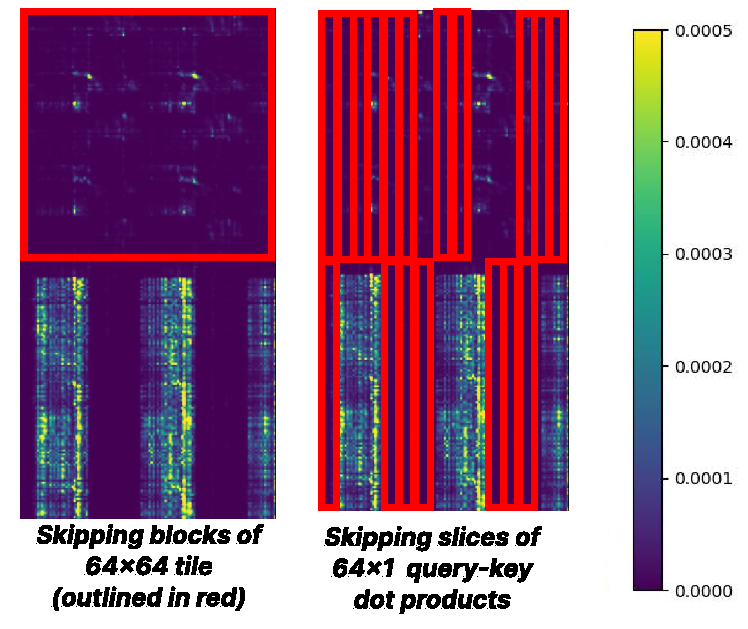
\includegraphics[width=1.0\linewidth]{fig/fig5.pdf}

   \caption{Attention weight visualization of the proposed temporal weighted attention.Darker colors indicate a higher level of attention toward the corresponding regions.}
   \label{fig5}
\end{figure}
\vspace{-3pt}
\begin{figure}[htbp]
  \centering
  % \fbox{\rule{0pt}{2in} \rule{2\linewidth}{0pt}}
    \includegraphics[width=1.0\linewidth]{fig/fig4.pdf}

   \caption{Visualization of online action detection. The curves indicate the predicted probability of the ground-truth class (Cricket Shot) with baseline and our method.}
   \label{fig4}
\end{figure}
\begin{figure*}[htbp]
  \centering
  % \fbox{\rule{0pt}{2in} \rule{0.8\linewidth}{0pt}}
    \includegraphics[width=0.8\linewidth]{fig/fig_q.pdf}

   \caption{Visualization of the anticipation results of our method and the baseline. The incorrect anticipations are marked in red. }
   \label{fig3}
\end{figure*}
\subsection{Attention Visualization}
Fig. 7 illustrates the dynamic visualization of the proposed temporal weighted attention mechanism in extracting critical states for effective action understanding. In this figure, the second \textit{Squeeze cloth} is critical frame related action. Therefore, this action is the anchor for constructing critical state. In this instance, the temporal weighted attention assigns diminishing weights to frames as their temporal distance from the critical frame increases. This ensures that the model focuses primarily on the critical moment and its immediate context, prioritizing key cues that define the action while reducing the influence of distant, less relevant frames. Additionally, the temporal weighted attention mechanism extends beyond linear temporal dependencies. It is capable of discovering non-linear relationships by linking semantically similar frames across the sequence, even if they are temporally distant. For instance, frames associated with repeated instances of \textit{Squeeze cloth}, although separated in time, are given higher attention scores due to their shared action semantics. This ability to bridge temporally distant but semantically relevant frames enhances the model's understanding of complex action patterns and facilitates the construction of robust critical states.In this process, the mechanism not only condenses the sequence into key actionable insights but also ensures that the extracted critical states are rich in context, serving as a solid foundation for subsequent state relation modeling. 
% By dynamically prioritizing frames that encapsulate meaningful information and suppressing irrelevant information, the temporal weighted attention mechanism strengthens the model’s capacity to represent and model intricate action dynamics effectively.
\subsection{Qualitative Comparison.}
We qualitatively analyze the performance of our proposed method for online action detection and action anticipation. In this section, we select MAT\cite{wang2023memory} as the baseline method.

Fig. 8 showcases a qualitative comparison between our method and baseline on the current action category from the THUMOS'14 dataset. The y-axis represents the probability of predicting the current action (Cricket Shot). Our model (red curve) demonstrates superior performance in detecting action compared to baseline (blue curve).Notably, our method effectively suppresses background frame noise and produces higher confidence scores during action period. The figure illustrates our model's ability to maintain stable predictions throughout the action duration. At the beginning and end of each \textit{Cricket Shot} action, our model provides sharp transitions, minimizing false positives in the background regions. This improvement highlights the robustness of our approach in isolating critical moments and reducing ambiguity during action transitions. This qualitative analysis underscores the advantages of our method in real-world scenarios, where precise identification of action boundaries is critical for downstream tasks.

Fig. 9 shows action anticipation results produced by our method on the EPIC-Kitchens dataset. Both successful and erroneous predictions are illustrated to provide comprehensive insights. In the first two examples, for sequences with clearly action patterns, our method accurately anticipates the future actions. In the third example, following the action \textit{mix coconut milk}, our method correctly anticipates the action \textit{add water}, whereas the baseline incorrectly predicts \textit{put down bowl}. This is due to our approach's capability to learning multi-dimensional relationships between actions, uncovering potential dependencies even among actions with lower similarity, rather than merely focusing on immediate temporal continuity as the baseline does. In the fourth example, our method incorrectly predicts the noun (\textit{potato} instead of \textit{pan}) while correctly capturing the intended verb (\textit{stir}). This suggests that although our model accurately understands action dynamics, it still has limitations in fine-grained semantic understanding. Addressing this semantic limitation represents a promising direction for future research. Finally, in the fifth example, both our method and the baseline predict \textit{open microwave} following the action \textit{pour food on plate}, whereas the ground truth is \textit{throw packaging}. Interestingly, the predicted action (\textit{open microwave}) indeed occurs shortly after the ground-truth action (\textit{throw packaging}). Such spontaneous actions posing significant challenges. In such cases, accurate prediction is challenging for the model, and even humans may make mistakes.
\section{Conclusion}
This study has presented the SSM, an innovative framework designed to unify action detection and anticipation tasks by effectively modeling dynamics and enabling cross-temporal interactions. Through the CSMC module, our model selectively captured critical states, reducing redundancy. The APL module constructs a ST graph by encoding multi-dimensional dependencies among critical states. Hence the action dynamics is represented and potential cue is generated. The CTI module models mutual influence between observed states and potential future cue, refining current and future representation to support online action detection and anticipation. Comprehensive evaluations across multiple benchmark datasets demonstrate the robustness generalization ability and superior performance of the proposed SSM framework, particularly in modeling complex, non-linear temporal relationships and accurately predicting intricate action transitions. Our findings highlight the importance of integrating critical states, diverse state-transition patterns, and cross-temporal interactions to advance action understanding.



% \section*{Acknowledgments}
% We thank Sulis (HPC facility) for providing computational resources to support this research.



% {\appendix[Proof of the Zonklar Equations]
% Use $\backslash${\tt{appendix}} if you have a single appendix:
% Do not use $\backslash${\tt{section}} anymore after $\backslash${\tt{appendix}}, only $\backslash${\tt{section*}}.
% If you have multiple appendixes use $\backslash${\tt{appendices}} then use $\backslash${\tt{section}} to start each appendix.
% You must declare a $\backslash${\tt{section}} before using any $\backslash${\tt{subsection}} or using $\backslash${\tt{label}} ($\backslash${\tt{appendices}} by itself
%  starts a section numbered zero.)}



%{\appendices
%\section*{Proof of the First Zonklar Equation}
%Appendix one text goes here.
% You can choose not to have a title for an appendix if you want by leaving the argument blank
%\section*{Proof of the Second Zonklar Equation}
%Appendix two text goes here.}



% \section{References Section}
% You can use a bibliography generated by BibTeX as a .bbl file.
%  BibTeX documentation can be easily obtained at:
%  http://mirror.ctan.org/biblio/bibtex/contrib/doc/
%  The IEEEtran BibTeX style support page is:
%  http://www.michaelshell.org/tex/ieeetran/bibtex/
 
%  % argument is your BibTeX string definitions and bibliography database(s)

% %
% \section{Simple References}
% You can manually copy in the resultant .bbl file and set second argument of $\backslash${\tt{begin}} to the number of references
%  (used to reserve space for the reference number labels box).

% \begin{thebibliography}{1}
\bibliographystyle{IEEEtran}
\bibliography{tmm_manuscript}
% \bibitem{ref1}
% {\it{Mathematics Into Type}}. American Mathematical Society. [Online]. Available: https://www.ams.org/arc/styleguide/mit-2.pdf

% \bibitem{ref2}
% T. W. Chaundy, P. R. Barrett and C. Batey, {\it{The Printing of Mathematics}}. London, U.K., Oxford Univ. Press, 1954.

% \bibitem{ref3}
% F. Mittelbach and M. Goossens, {\it{The \LaTeX Companion}}, 2nd ed. Boston, MA, USA: Pearson, 2004.

% \bibitem{ref4}
% G. Gr\"atzer, {\it{More Math Into LaTeX}}, New York, NY, USA: Springer, 2007.

% \bibitem{ref5}M. Letourneau and J. W. Sharp, {\it{AMS-StyleGuide-online.pdf,}} American Mathematical Society, Providence, RI, USA, [Online]. Available: http://www.ams.org/arc/styleguide/index.html

% \bibitem{ref6}
% H. Sira-Ramirez, ``On the sliding mode control of nonlinear systems,'' \textit{Syst. Control Lett.}, vol. 19, pp. 303--312, 1992.

% \bibitem{ref7}
% A. Levant, ``Exact differentiation of signals with unbounded higher derivatives,''  in \textit{Proc. 45th IEEE Conf. Decis.
% Control}, San Diego, CA, USA, 2006, pp. 5585--5590. DOI: 10.1109/CDC.2006.377165.

% \bibitem{ref8}
% M. Fliess, C. Join, and H. Sira-Ramirez, ``Non-linear estimation is easy,'' \textit{Int. J. Model., Ident. Control}, vol. 4, no. 1, pp. 12--27, 2008.

% \bibitem{ref9}
% R. Ortega, A. Astolfi, G. Bastin, and H. Rodriguez, ``Stabilization of food-chain systems using a port-controlled Hamiltonian description,'' in \textit{Proc. Amer. Control Conf.}, Chicago, IL, USA,
% 2000, pp. 2245--2249.

% \end{thebibliography}


% \newpage

% \section{Biography Section}
% If you have an EPS/PDF photo (graphicx package needed), extra braces are
%  needed around the contents of the optional argument to biography to prevent
%  the LaTeX parser from getting confused when it sees the complicated
%  $\backslash${\tt{includegraphics}} command within an optional argument. (You can create
%  your own custom macro containing the $\backslash${\tt{includegraphics}} command to make things
%  simpler here.)
 
% \vspace{11pt}

% \bf{If you include a photo:}\vspace{-33pt}
% \begin{IEEEbiography}[{\includegraphics[width=1in,height=1.25in,clip,keepaspectratio]{fig1}}]{Michael Shell}
% Use $\backslash${\tt{begin\{IEEEbiography\}}} and then for the 1st argument use $\backslash${\tt{includegraphics}} to declare and link the author photo.
% Use the author name as the 3rd argument followed by the biography text.
% \end{IEEEbiography}

% \vspace{11pt}

% \bf{If you will not include a photo:}\vspace{-33pt}
% \begin{IEEEbiographynophoto}{John Doe}
% Use $\backslash${\tt{begin\{IEEEbiographynophoto\}}} and the author name as the argument followed by the biography text.
% \end{IEEEbiographynophoto}




\vfill

\end{document}


